% Requires: \usepackage{subcaption} \usepackage{graphicx}
% Image paths are relative to this .tex file's location.
% Generated by: smixae latex figures  (experiment: gemma_2_9b_l11, newline)

\begin{figure*}[t]
\centering
\begin{minipage}[c]{0.88\linewidth}
\centering
  \begin{subfigure}[t]{0.49\linewidth}
    \centering
    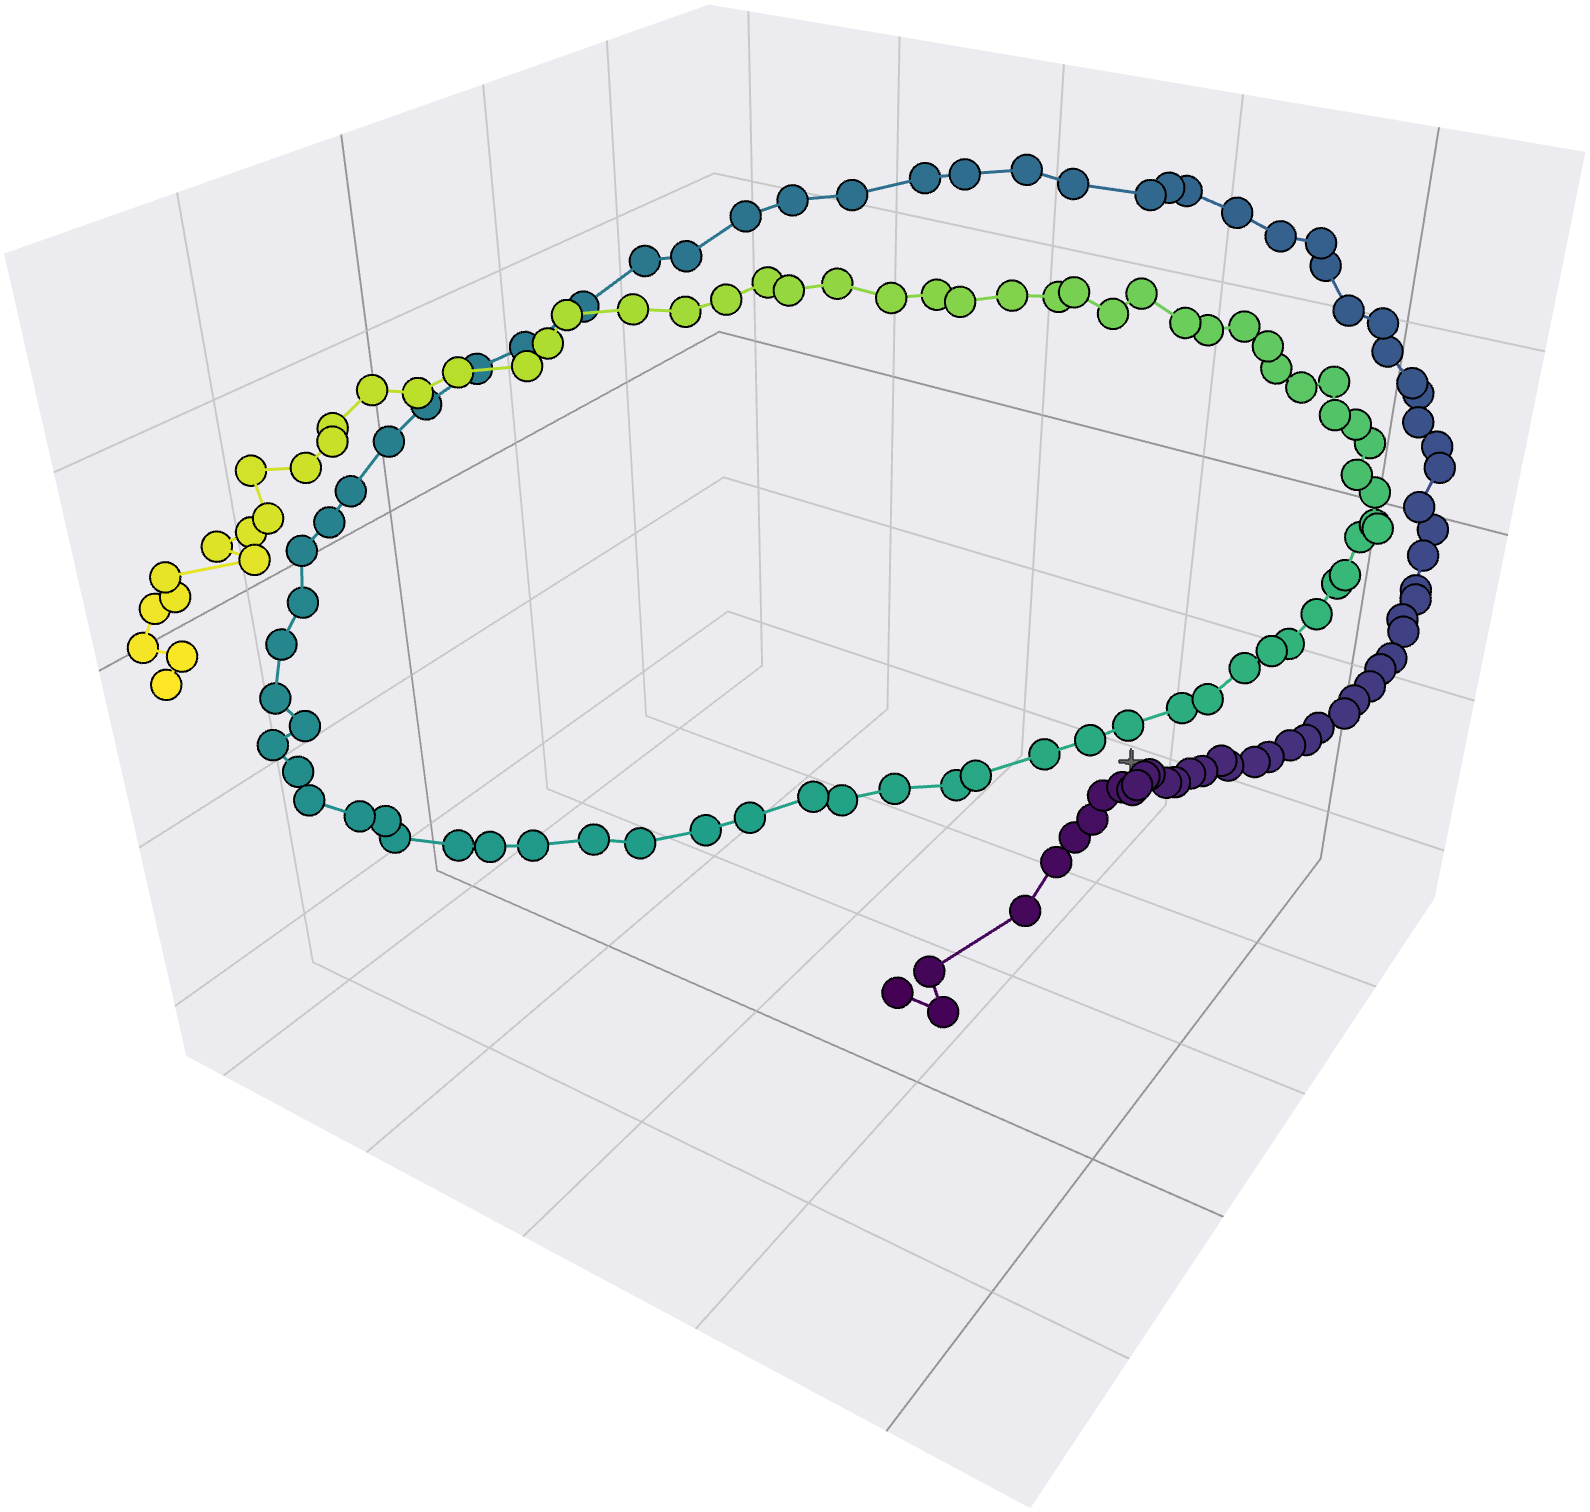
\includegraphics[width=\linewidth]{camera_ready/gemma_2_9b_l11__pile-uncopyrighted__E541__periodic_gain__per_gain__0.5668__means.png}
    \caption{E541, Periodic Gain ($\Delta$per\,=\,0.567)}
  \end{subfigure}
  \hfill
  \begin{subfigure}[t]{0.49\linewidth}
    \centering
    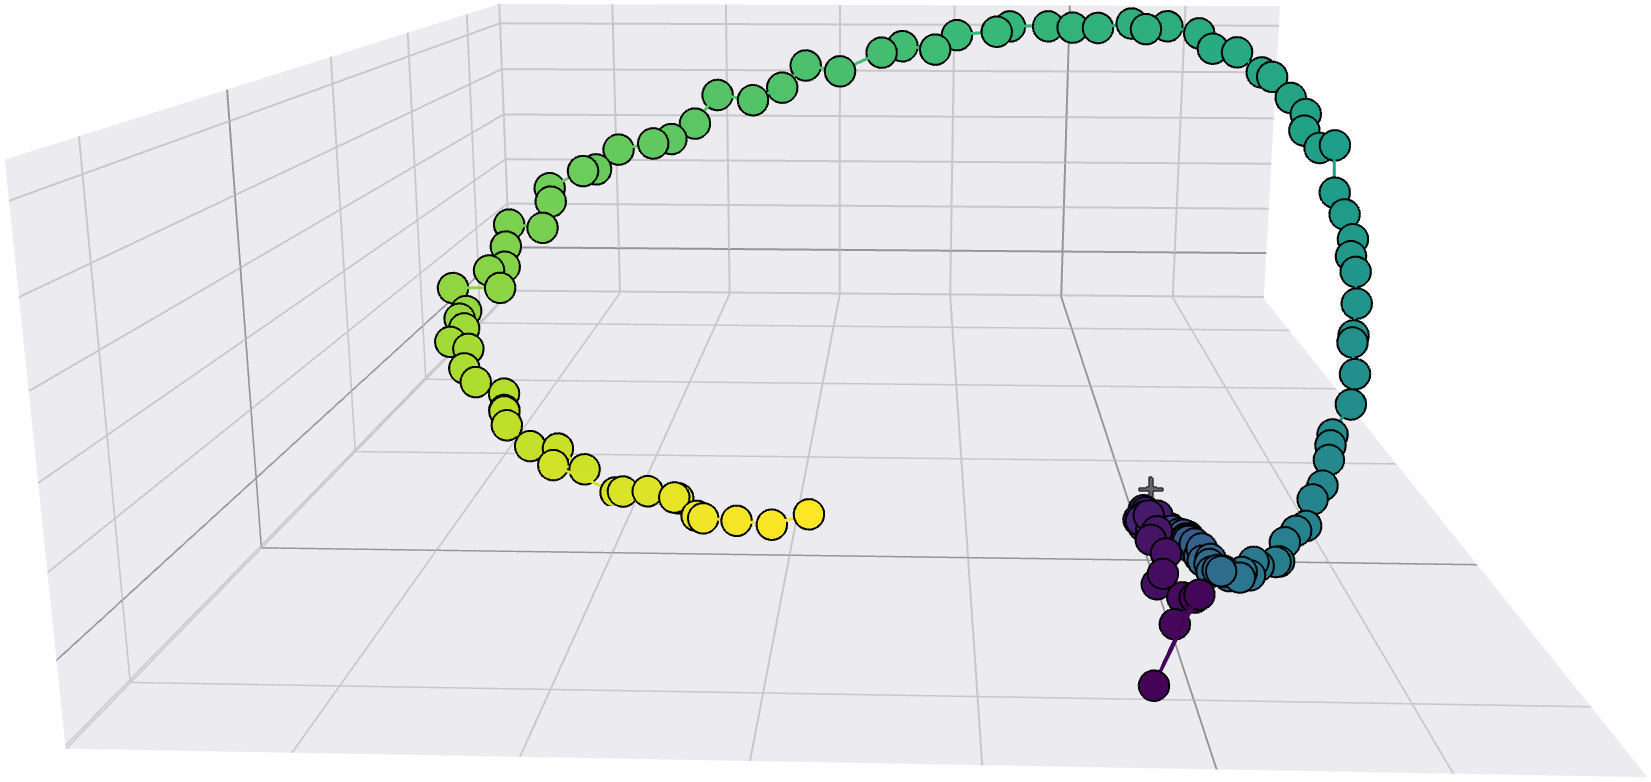
\includegraphics[width=\linewidth]{camera_ready/gemma_2_9b_l11__pile-uncopyrighted__E1521__periodic_gain__per_gain__0.4970__means.png}
    \caption{E1521, Periodic Gain ($\Delta$per\,=\,0.497)}
  \end{subfigure}
\end{minipage}\hfill
\begin{minipage}[c]{0.10\linewidth}
  \centering
  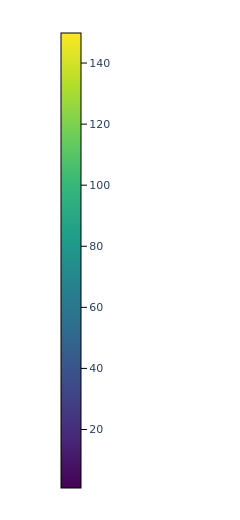
\includegraphics[width=\linewidth]{legends/legend_pile-uncopyrighted__150.png}
\end{minipage}
\caption{Newline Position (150 chars) --- Gemma 2 9B, Layer 11.}
\end{figure*}

